\documentclass[12pt]{article}
\usepackage[margin=1in]{geometry}
\usepackage{setspace}
\onehalfspacing

% Start of preamble
%==========================================================================================%
% Required to support mathematical unicode
\usepackage[warnunknown, fasterrors, mathletters]{ucs}
\usepackage[utf8x]{inputenc}

\usepackage[dvipsnames,table,xcdraw]{xcolor}
\usepackage{hyperref} 
\hypersetup{
colorlinks=true,
linkcolor=blue,
filecolor=magenta,
urlcolor=cyan,
pdfpagemode=FullScreen
}

% Standard mathematical typesetting packages
\usepackage{amsmath,amssymb,amscd,amsthm,amsxtra, pxfonts}
\usepackage{mathtools,mathrsfs,dsfont,xparse}

% Symbol and utility packages
\usepackage{cancel, textcomp}
\usepackage[mathscr]{euscript}
\usepackage[nointegrals]{wasysym}
\usepackage{apacite}

% Extras
\usepackage{physics}  
\usepackage{tikz-cd} 
\usepackage{microtype}
\usepackage{enumitem}
\usepackage{titling}
\usepackage{graphicx}

% Fancy theorems due to @intuitively on discord
\usepackage{mdframed}
\newmdtheoremenv[
backgroundcolor=NavyBlue!30,
linewidth=2pt,
linecolor=NavyBlue,
topline=false,
bottomline=false,
rightline=false,
innertopmargin=10pt,
innerbottommargin=10pt,
innerrightmargin=10pt,
innerleftmargin=10pt,
skipabove=\baselineskip,
skipbelow=\baselineskip
]{mytheorem}{Theorem}

\newenvironment{theorem}{\begin{mytheorem}}{\end{mytheorem}}

\newtheorem{corollary}{Corollary}
\newtheorem{lemma}{Lemma}

\newtheoremstyle{definitionstyle}
{\topsep}%
{\topsep}%
{}%
{}%
{\bfseries}%
{.}%
{.5em}%
{}%
\theoremstyle{definitionstyle}
\newmdtheoremenv[
backgroundcolor=Violet!30,
linewidth=2pt,
linecolor=Violet,
topline=false,
bottomline=false,
rightline=false,
innertopmargin=10pt,
innerbottommargin=10pt,
innerrightmargin=10pt,
innerleftmargin=10pt,
skipabove=\baselineskip,
skipbelow=\baselineskip,
]{mydef}{Definition}
\newenvironment{definition}{\begin{mydef}}{\end{mydef}}

\newtheorem*{remark}{Remark}

\newtheorem*{example}{Example}

% Common shortcuts
\def\mbb#1{\mathbb{#1}}
\def\mfk#1{\mathfrak{#1}}

\def\bN{\mbb{N}}
\def \C{\mbb{C}}
\def \R{\mbb{R}}
\def\bQ{\mbb{Q}}
\def\bZ{\mbb{Z}}
\def \cph{\varphi}
\renewcommand{\th}{\theta}
\def \ve{\varepsilon}
\newcommand{\mg}[1]{\| #1 \|}

% Often helpful macros
\newcommand{\floor}[1]{\left\lfloor#1\right\rfloor}
\newcommand{\ceil}[1]{\left\lceil#1\right\rceil}
\renewcommand{\qed}{\hfill\qedsymbol}
\renewcommand{\P}{\mathbb P\qty}
\newcommand{\E}{\mathbb{E}\qty}
\newcommand{\Cov}{\mathrm{Cov}\qty}
\newcommand{\Var}{\mathrm{Var}\qty}

% Sets
\usepackage{braket}

\graphicspath{{/}}
\usepackage{float}

\newcommand{\SET}[1]{\Set{\mskip-\medmuskip #1 \mskip-\medmuskip}}

% End of preamble
%==========================================================================================%

% Start of commands specific to this file
%==========================================================================================%

%==========================================================================================%
% End of commands specific to this file

\title{CSE 446 HW3}
\date{\today}
\author{Rohan Mukherjee}

\begin{document}
    \maketitle
    \subsection*{A1.}
    \begin{enumerate}[label=(\alph*)]
        \item In general deep neural networks are non-linear optimization problems, and often times tend to be non-convex and have many local minima. Gradient descent provides great results but not provably (nor likely) the best.
        \item When training deep neural networks, it is much better to initialize the weights according to some random uniform distribution, instead of all zeros because all zeros could get stuck immediately in local mimina and not be able to escape them with gradient descent.
        \item Yes, using non-linear activation functions allows the model to be much more complex and have non-linear decision boundaries. 
        \item No. Using DP and the theorem that calculating gradients can be done up to small constants in the same time complexity as just evaluating a function, backpropogation runs in the same time complexity as the forward pass.
        \item Sometimes neural networks can be too complex leading to too much bias, or simply have too many parameters to train in a reasonable amount of time. In this case the neural network may not be the best model to use. 
    \end{enumerate}

    \subsection*{A2.}
    Notice that,
    \begin{align*}
        K(x,x') &= \sum_{i=0}^\infty \frac{1}{\sqrt{i!}} e^{-x^2/2}x^i \cdot \frac{1}{\sqrt{i!}} e^{-x'^2/2}x'^i = \sum_{i=0}^\infty \frac{1}{i!} e^{-(x^2+x'^2)/2} \cdot (xx')^i \\
        &= e^{-(x^2+x'^2)/2} \cdot e^{xx'} = e^{-(x^2+x'^2-2xx')/2} = e^{-(x-x')^2/2}
    \end{align*}
    Where we used that,
    \begin{align*}
        e^x = \sum_{i=0}^\infty \frac{x^i}{i!}
    \end{align*}

    \subsection*{A3.}
    The optimal hyperparameters used are in the title of the below graphs:
    \begin{figure}[H]
        \centering
        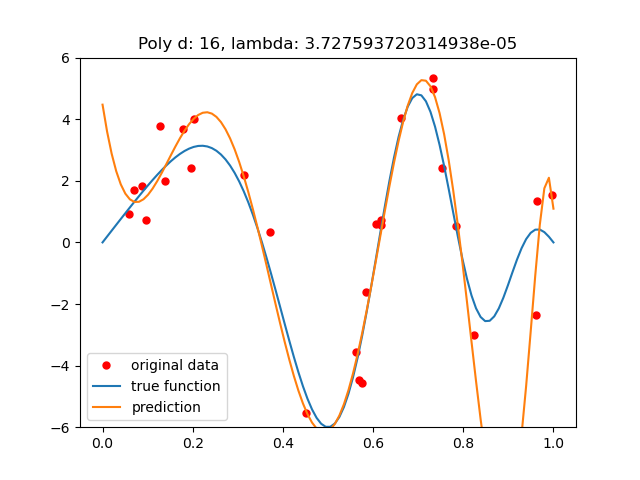
\includegraphics[width=0.5\textwidth]{kernels_poly.png}
        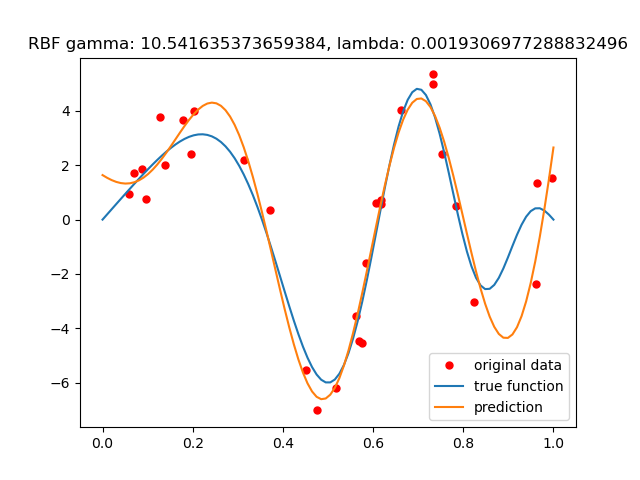
\includegraphics[width=0.5\textwidth]{kernels_rbf.png}
    \end{figure}

    \subsection*{A4.}
    \begin{enumerate}
        \item[b.] Here are the plots of the train and validation set losses for each loss function:
        \begin{figure}[H]
            \centering
            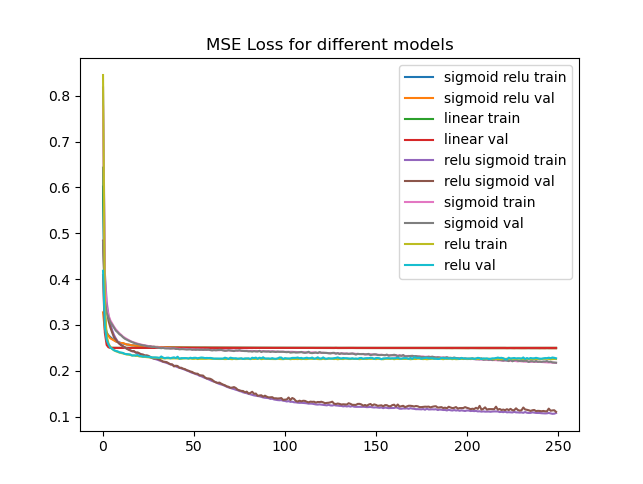
\includegraphics[width=0.8\textwidth]{mse_images.png}
            \includegraphics*[width=0.8\textwidth]{ce_images.png}
        \end{figure}
        \item[c.] The best performing architectures are seen from above to be relu sigmoid in both cases. It is honestly a little shocking how much it leaves the competition in the dust! Here are the accuracy plots for each:
        \begin{figure}[H]
            \centering
            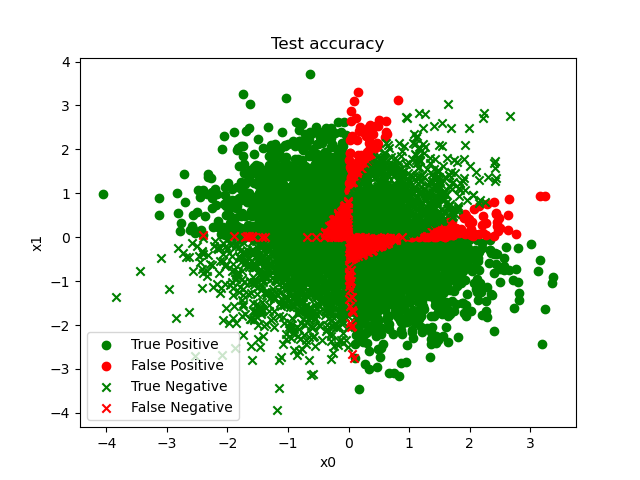
\includegraphics[width=0.7\textwidth]{mse_acc.png}
            \caption{MSE}
            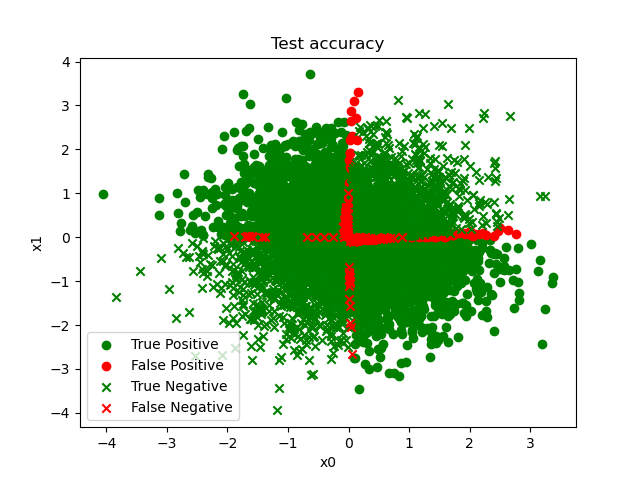
\includegraphics[width=0.7\textwidth]{ce_acc.png}
            \caption{Cross Entropy}
        \end{figure}
    \end{enumerate}

    \subsection*{A5.}
    \begin{enumerate}[label=(\alph*)]
        \item I get an accuracy of 0.97557\% and a loss of 0.0816\% on the test data. Here is the graph of the training loss:
        \begin{figure}[H]
            \centering
            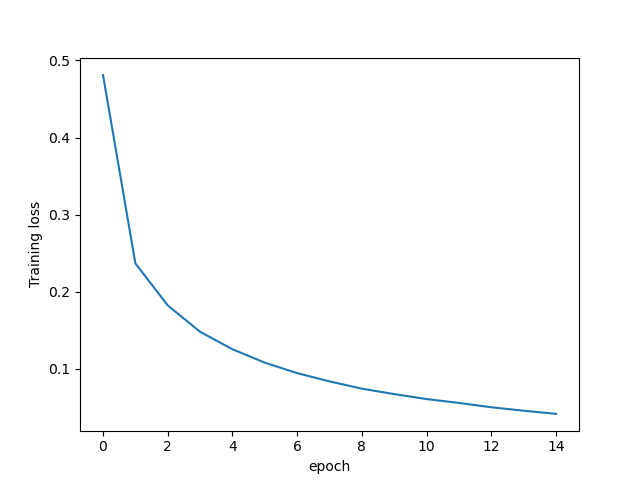
\includegraphics[width=0.5\textwidth]{F1_training_loss.png}
        \end{figure}
        \item On the test data, after training to 99\% accuracy on the training data, I get an accuracy of 96.668\% and a loss of 0.113. The graph I get is as follows:
        \begin{figure}[H]
            \centering
            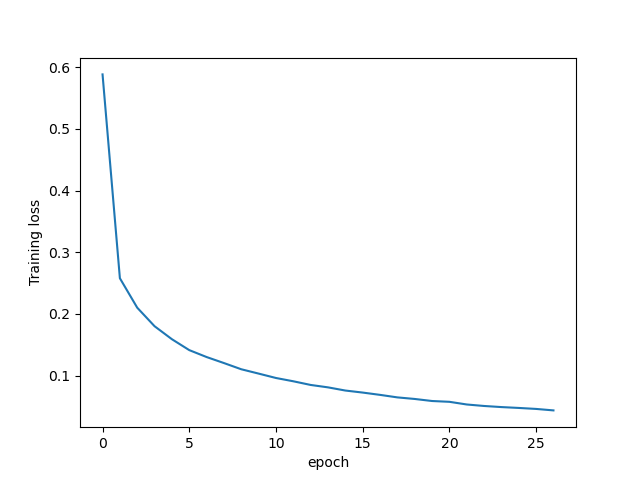
\includegraphics[width=0.5\textwidth]{F2_training_loss.png}
        \end{figure}

        \item The first model, F1, has 50,890 parameters while the second has only 26,506 parameters. The first one is seen to perform better as per the above stats. I believe this is because it has a lot more parameters and thus can train a more complex model, yielding a higher accuracy. One would guess that if you have more complexity then you would be better able to represent the data.
    \end{enumerate}

    \subsection*{A6.}
    This homework assignment took me significantly longer than the previous, probably around 25-30 hours. I really enjoyed it!
\end{document}